\section{Signal MC}
\label{sec:signal_mc}
In order to study the efficiency of the event selection and the optimal opening angle for a Galactic center search, a signal monte carlo of 200,000 electromagnetic shower events was produced, with electron energies ranging from 30 MeV to 1 TeV.  The MC was split into 4 energy ranges: 30 MeV-1 GeV, 1 GeV-10 GeV, 10 GeV-100 GeV, and 100 GeV to 1 TeV.  Fifty thousand events were produced in each energy range, with a flat linear energy spectrum in each range.  Event positions within the detector were randomly selected uniformly within a cylinder 1 meter inside the wall of the inner detector, in order to account for migration of events in the fiducial volume, which is 2 meters inside the wall of the inner detector.  

The direction of the electromagnetic showers was chosen assuming the NFW annihilation model.  For each event, a random direction in equatorial coordinates was choosen so that the probability of an event's source being placed at an angle $\theta_\textrm{GC}$ from the galactic center is proportional to $\mathcal{J}_\textrm{ann}(\theta_{\textrm{GC}}) \sin \theta_{\textrm{GC}}$.  The $\sin \theta_{\textrm{GC}}$ factor is a geometrical affect.  Note that we are simulating a case where the scattered electrons direction is exactly parallel to the direction of the boosted dark matter.  While there would be expected to be some model dependent smearing of the boosted dark matter direction to the electron direction, the scattering is expected to be strongly peaked in the forward direction \cite{Agashe:2014yua}.  Thus, since it both has a minimal effect and is model dependent, the effect of this scattering directional smearing in ignored in the production of the signal MC.  In order to transform from equatorial coordinates to the horizontal coordinates of the detector, a random time is chosen for each event.  These times are randomly distributed at times during 
\SK good data runs which are used in the analysis.  The time chosen for an event is then used to transform from equatorial to horizontal coordinates.  While the simulation is created assuming the NFW annihilation model, other models can be studied by reweighting each event by the ratio of the new models J-factor to the NFW annihilation J-factor:
\begin{equation}
w_{\textrm{Model X}}=\frac{\mathcal{J}_{\textrm{Model X}}(\theta_\textrm{GC})}{\mathcal{J}_{\textrm{NFW ann}}(\theta_\textrm{GC})}
\label{eq:model_weight}
\end{equation} 
The Model dependent smearing mentioned above can similarly be added back into the simulation by event reweighting.

The signal MC was run through the most of the full SK MC production process: Simulation (SKDETSIM), FC reduction (FCCOMB), reconstruction (APFIT), and ntuple creation (FILLNT,ROOT2ZBS).  The only portions of the full SK MC production process excluded were PC and UPMU reduction (since this in an FC only analysis), fiTQun reconstruction (since this analysis uses only APFIT variables), and neutron tagging.  Although neutron tagging is an extremely important part of this analysis, there are no simulated neutrons in the signal MC, so we can safely assume that the background rate of false positive neutron tags in the signal MC is the same as the background rate found in the atmospheric MC (1.8\%).

The angular and energy resolutions for events passing all selection and analysis cuts are shown in Figures \ref{fig:angular_res} and \ref{fig:energy_res}.  As can be seen in Figure \ref{fig:angular_res}, the angular resolution for these events is better than $3^\circ$ for all energy ranges.  The bias towards understating the energy in the high energy range (Figure \ref{fig:energy_res_high}) and long tail on the negative side is due to the detector becoming saturated for very high energy events.

The efficiency of the selection and analysis cuts is shown in Figure \ref{fig:eff}.  Efficiency is defined as the number of events passing a set of cuts divided by the number of events simulated in the fiducial volume.  This is not exactly equivalent to the fraction of events produced in the fiducial volume which pass all cuts, as some events will migrate into the fiducial volume to offset events migrating out of the fiducial volume.  The total efficiency of the analysis turns on around 100 MeV and stays above $90\%$ until around 5-10 GeV, and then remains above $80\%$ until around 50 GeV.  The main cause of the reduction of efficiency with energy is the loss of containment at high energies; many higher energy electromagnetic showers are able to penetrate from the FV into the OD, and so do not pass fully-contained cuts.

\begin{figure*}
	\centering
	\subfigure[E$_e$=30MeV-1GeV, $\sigma$=2.8$^\circ$]{
		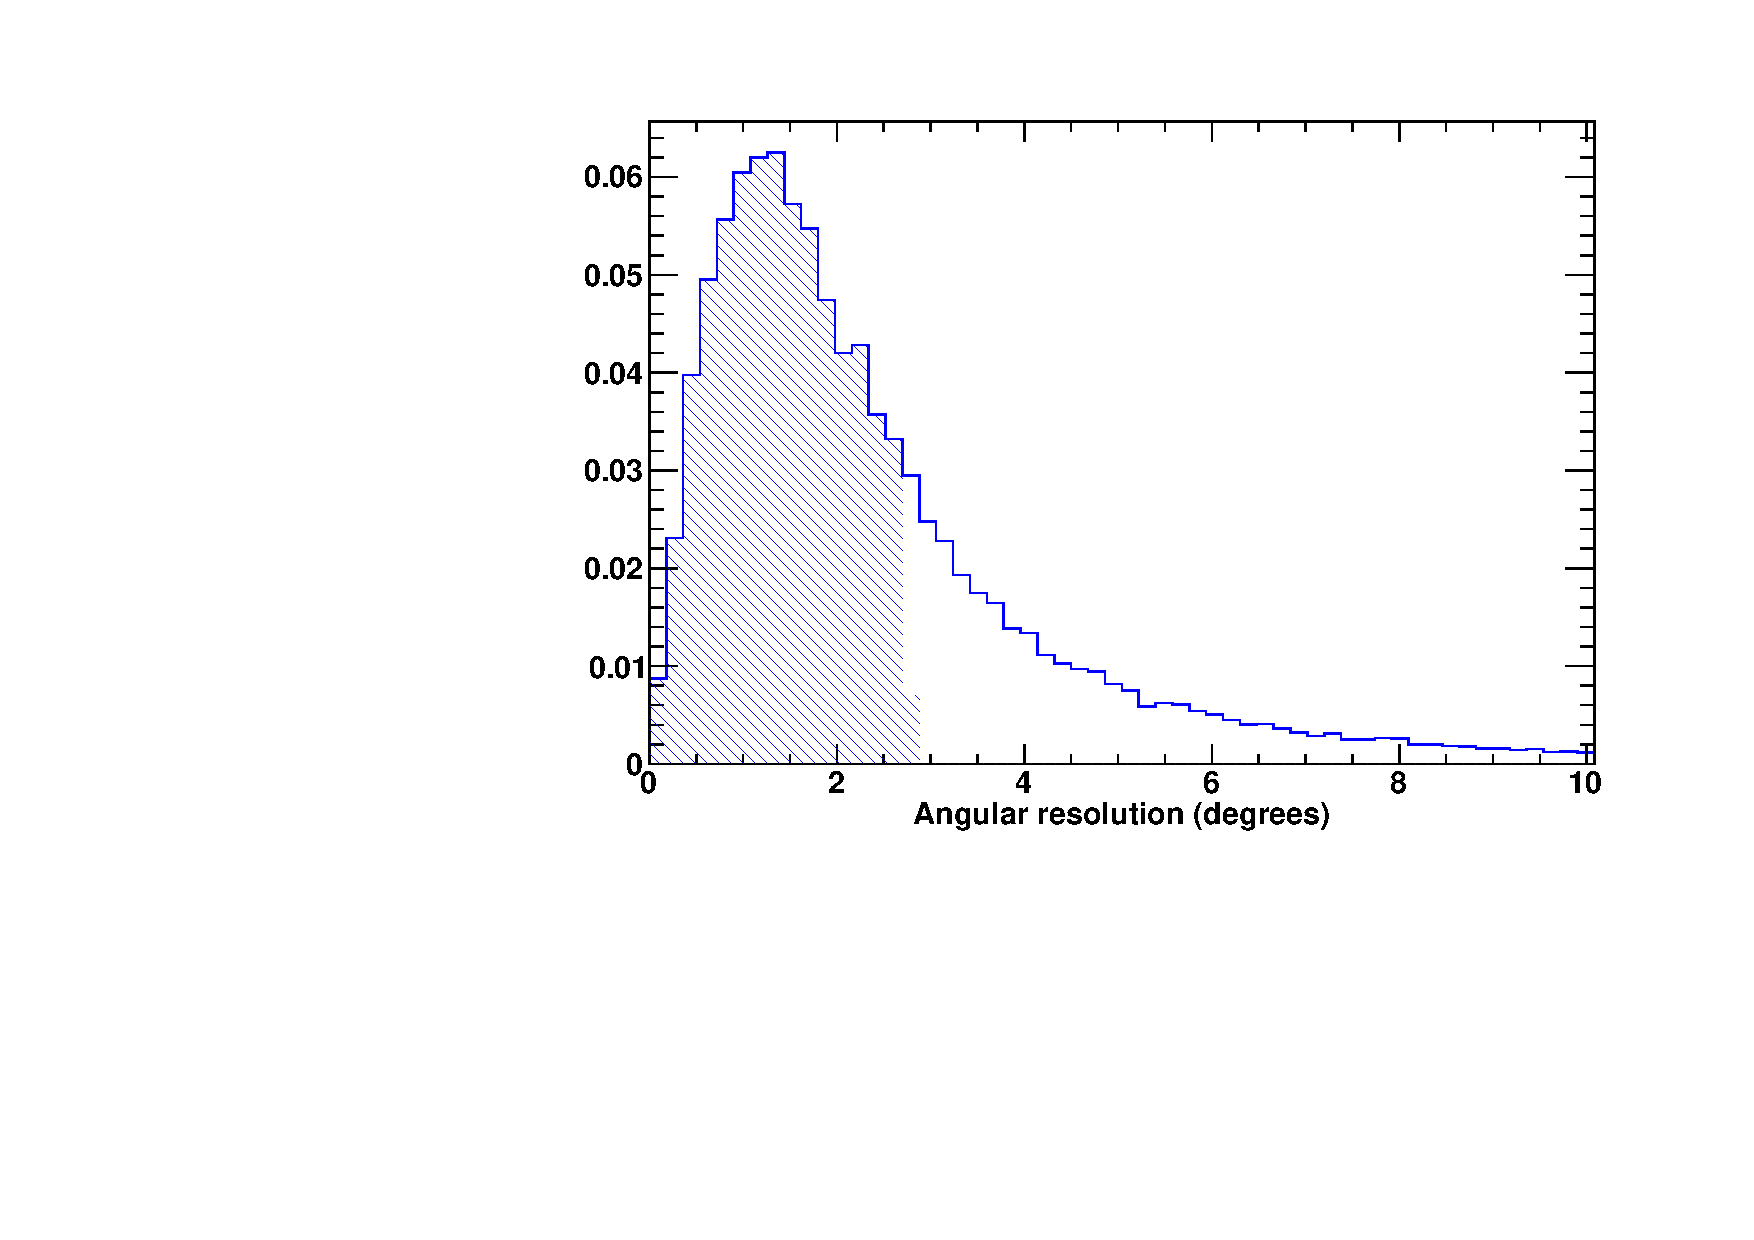
\includegraphics[width=0.3\textwidth]{figures/30MeV_1GeV_angular.pdf}
		\label{fig:angular_res_low}
	}
	\subfigure[E$_e$=1GeV-10GeV,$\sigma$=1.1$^\circ$]{
		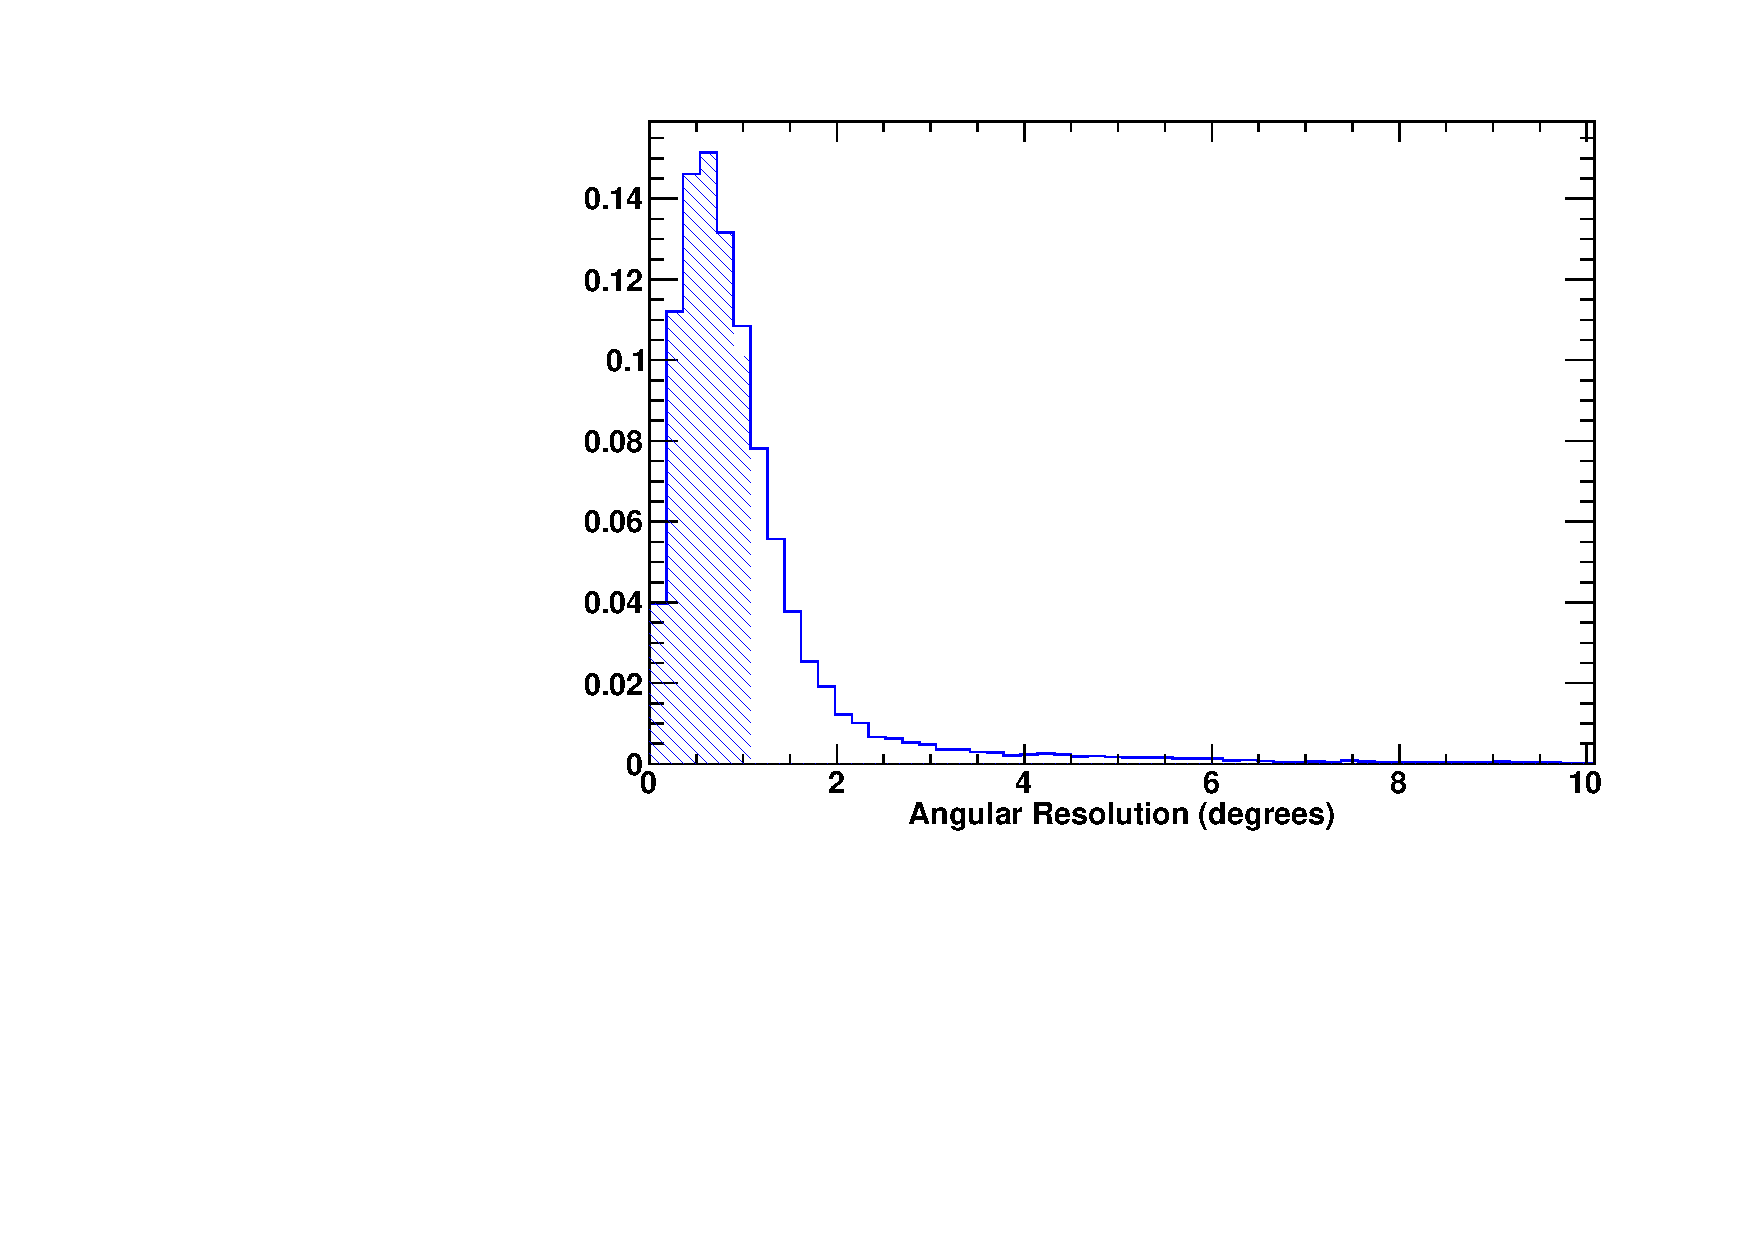
\includegraphics[width=0.3\textwidth]{figures/1GeV_10GeV_angular.pdf}
		\label{fig:angular_res_mid}
	}
	\subfigure[E$_e$=10GeV-100GeV,$\sigma$=2.3$^\circ$]{
		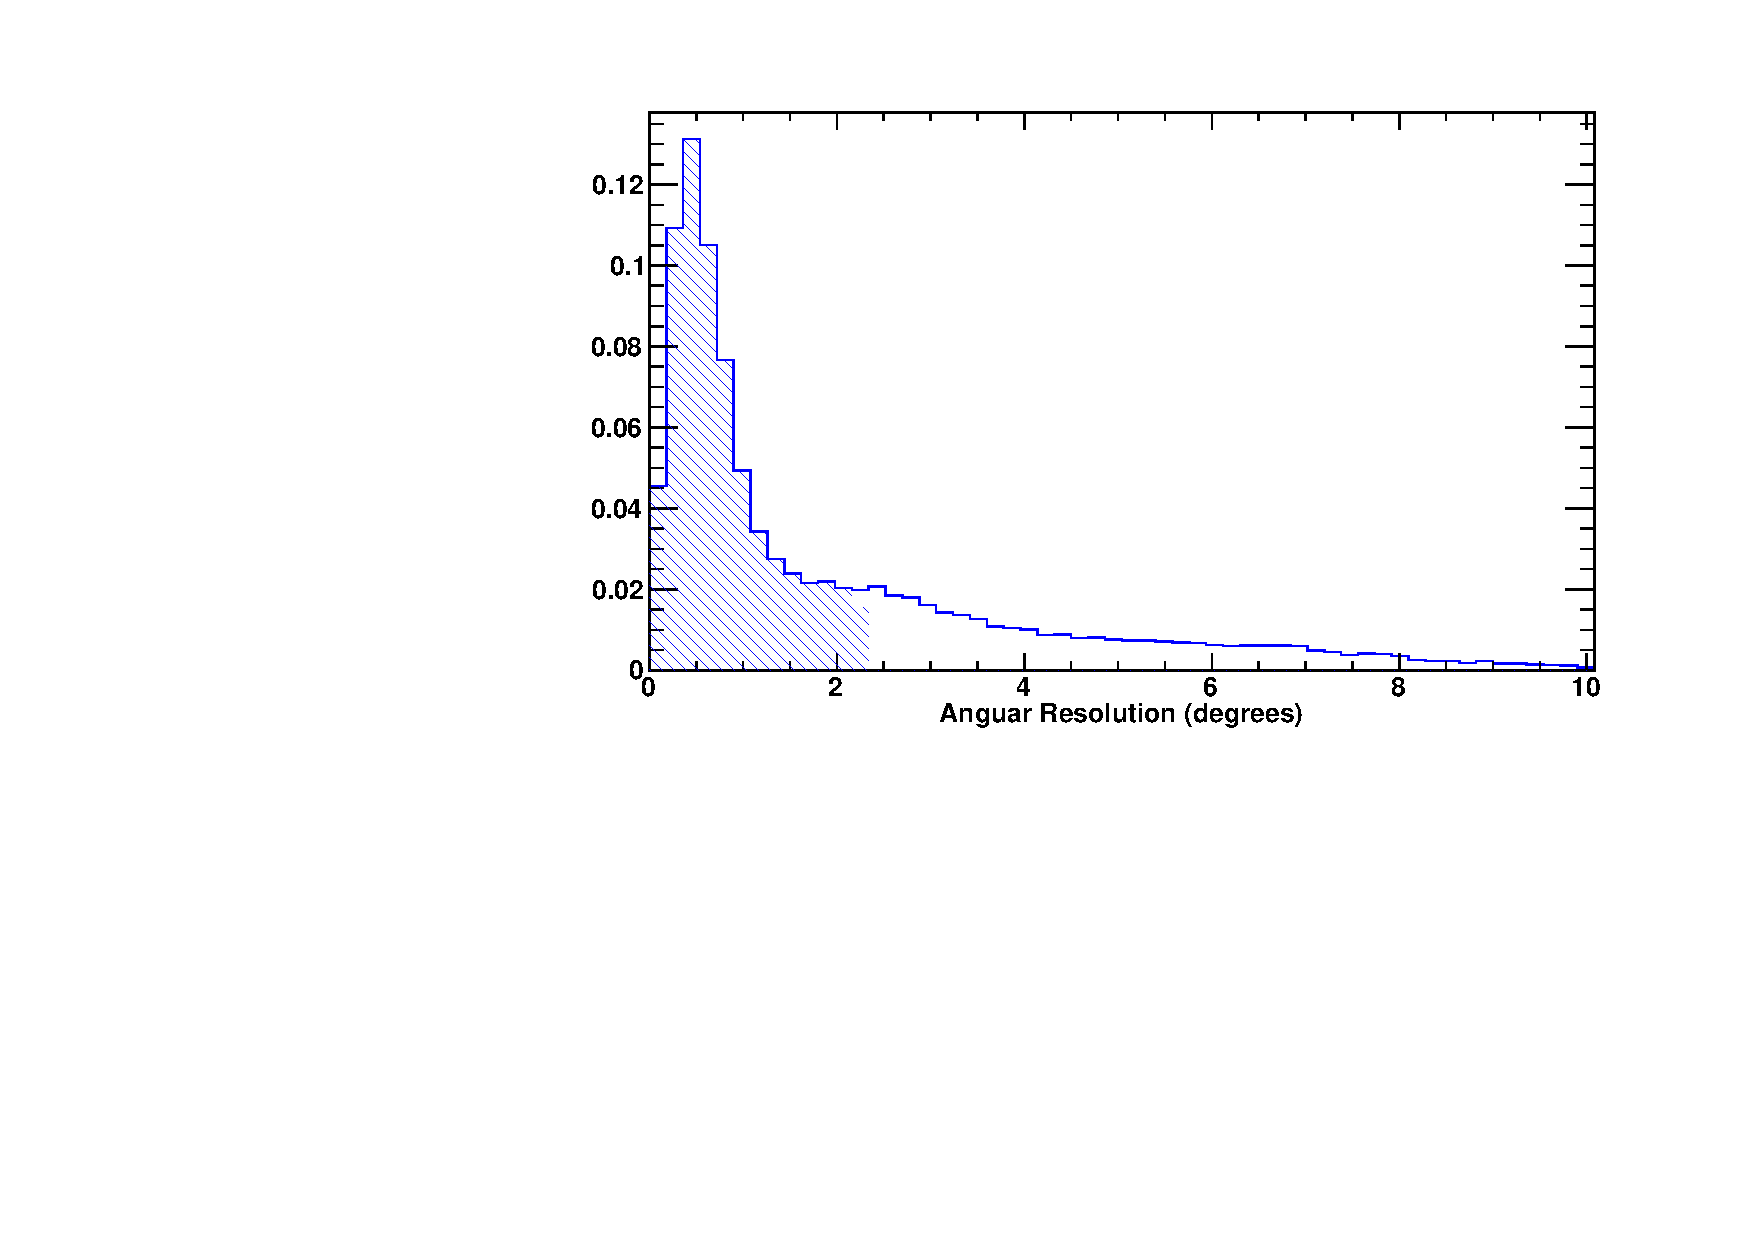
\includegraphics[width=0.3\textwidth]{figures/10GeV_100GeV_angular.pdf}
		\label{fig:angular_res_high}
	}
\caption{Angular resolution for events passing all selection and analysis cuts, from signal MC in 3 energy ranges.} 
\label{fig:angular_res}
\end{figure*}  

\begin{figure*}
	\centering
	\subfigure[E$_e$=30MeV-1GeV]{
		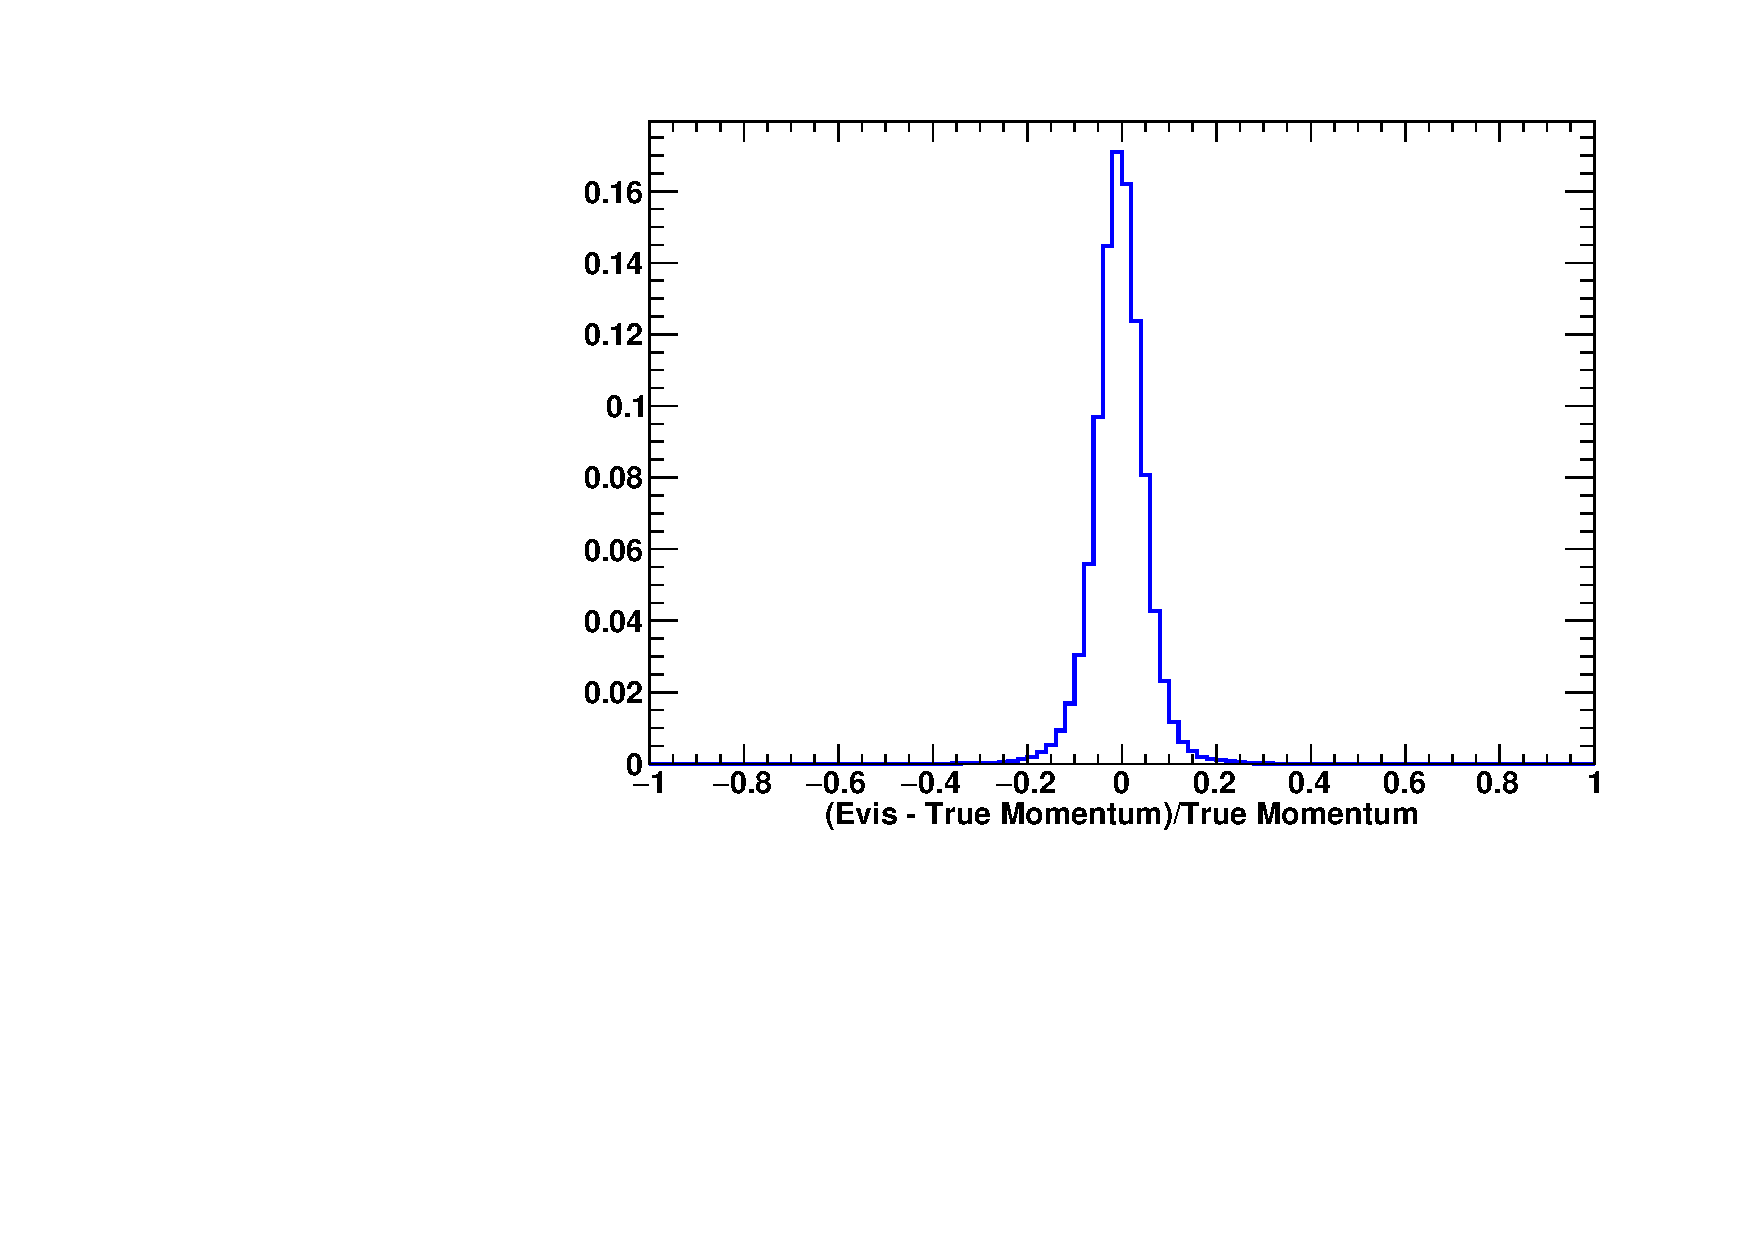
\includegraphics[width=0.3\textwidth]{figures/30MeV_1GeV_energy.pdf}
		\label{fig:energy_res_low}
	}
	\subfigure[E$_e$=1GeV-10GeV]{
		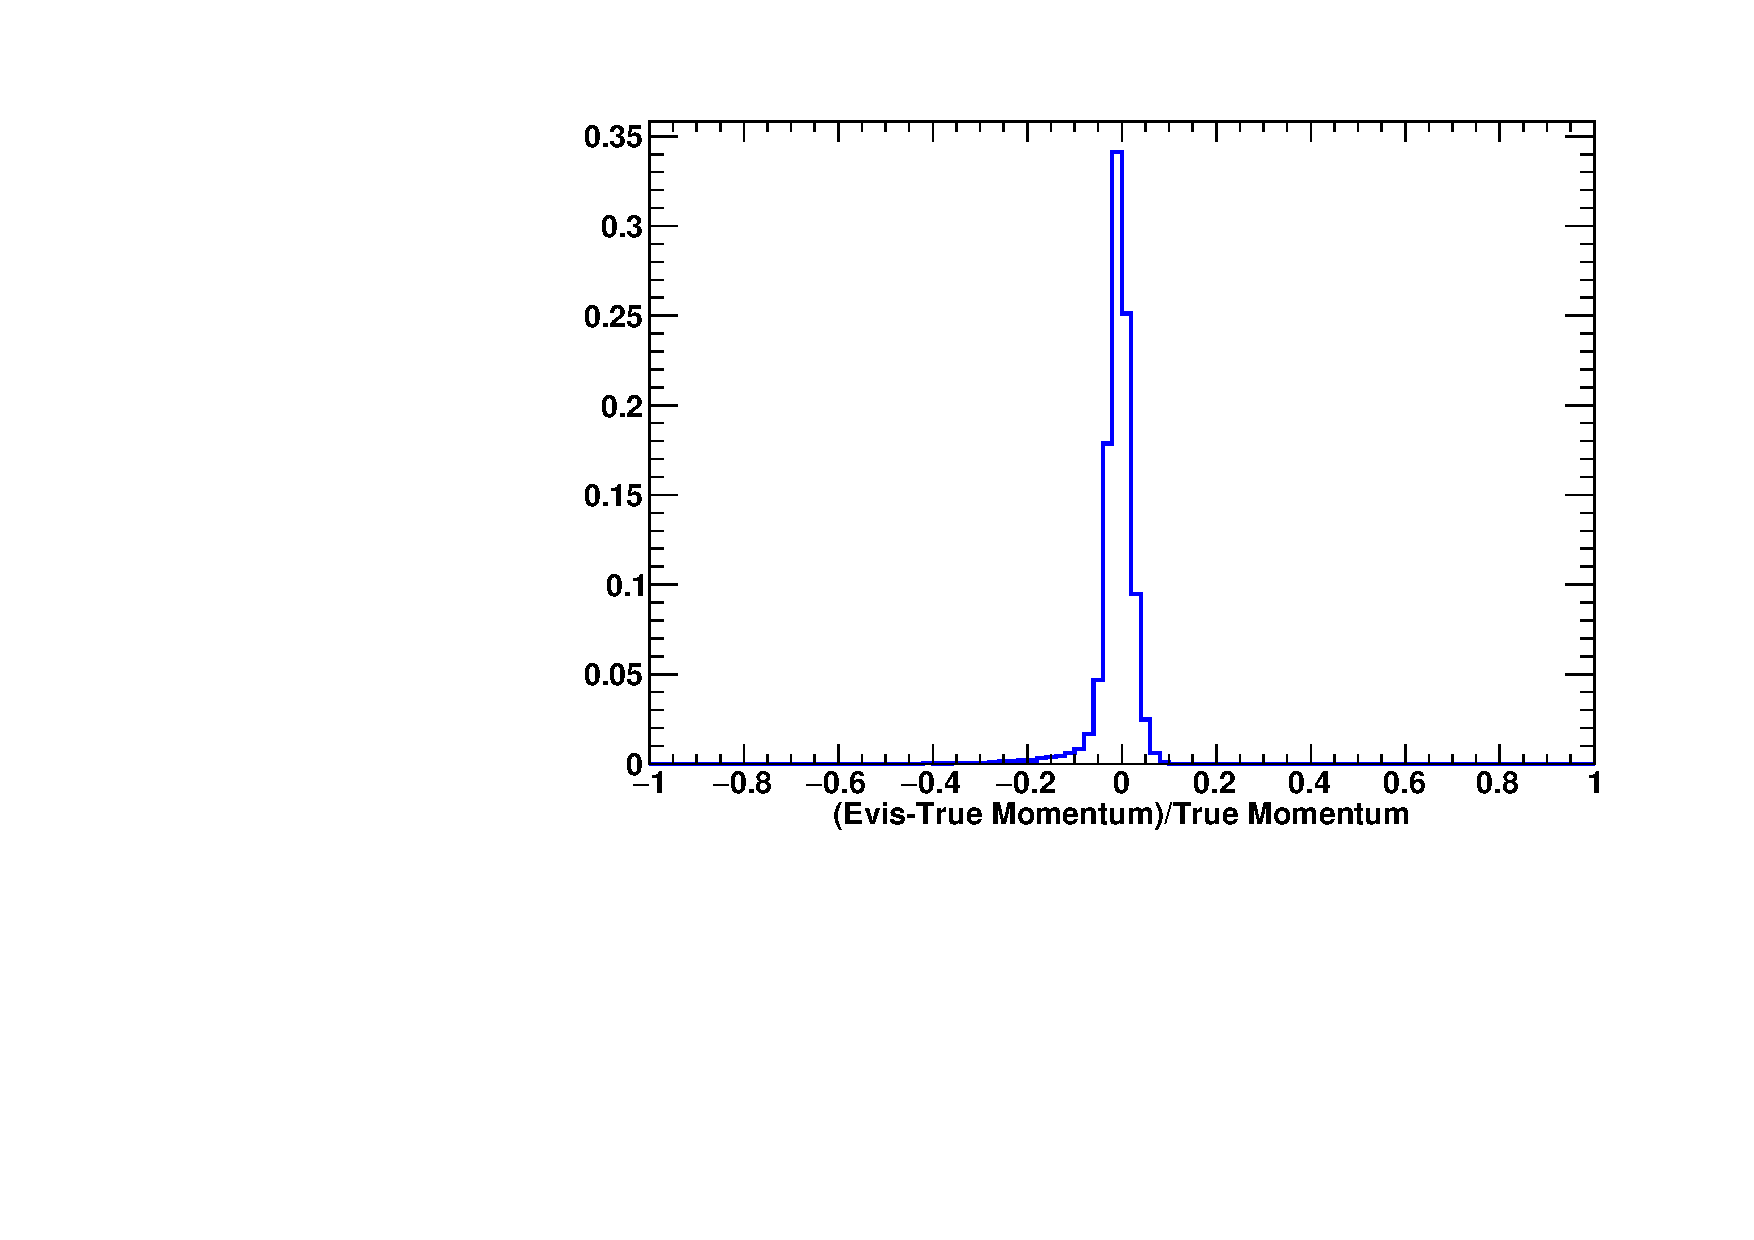
\includegraphics[width=0.3\textwidth]{figures/1GeV_10GeV_energy.pdf}
		\label{fig:energy_res_mid}
	}
	\subfigure[E$_e$=10GeV-100GeV]{
		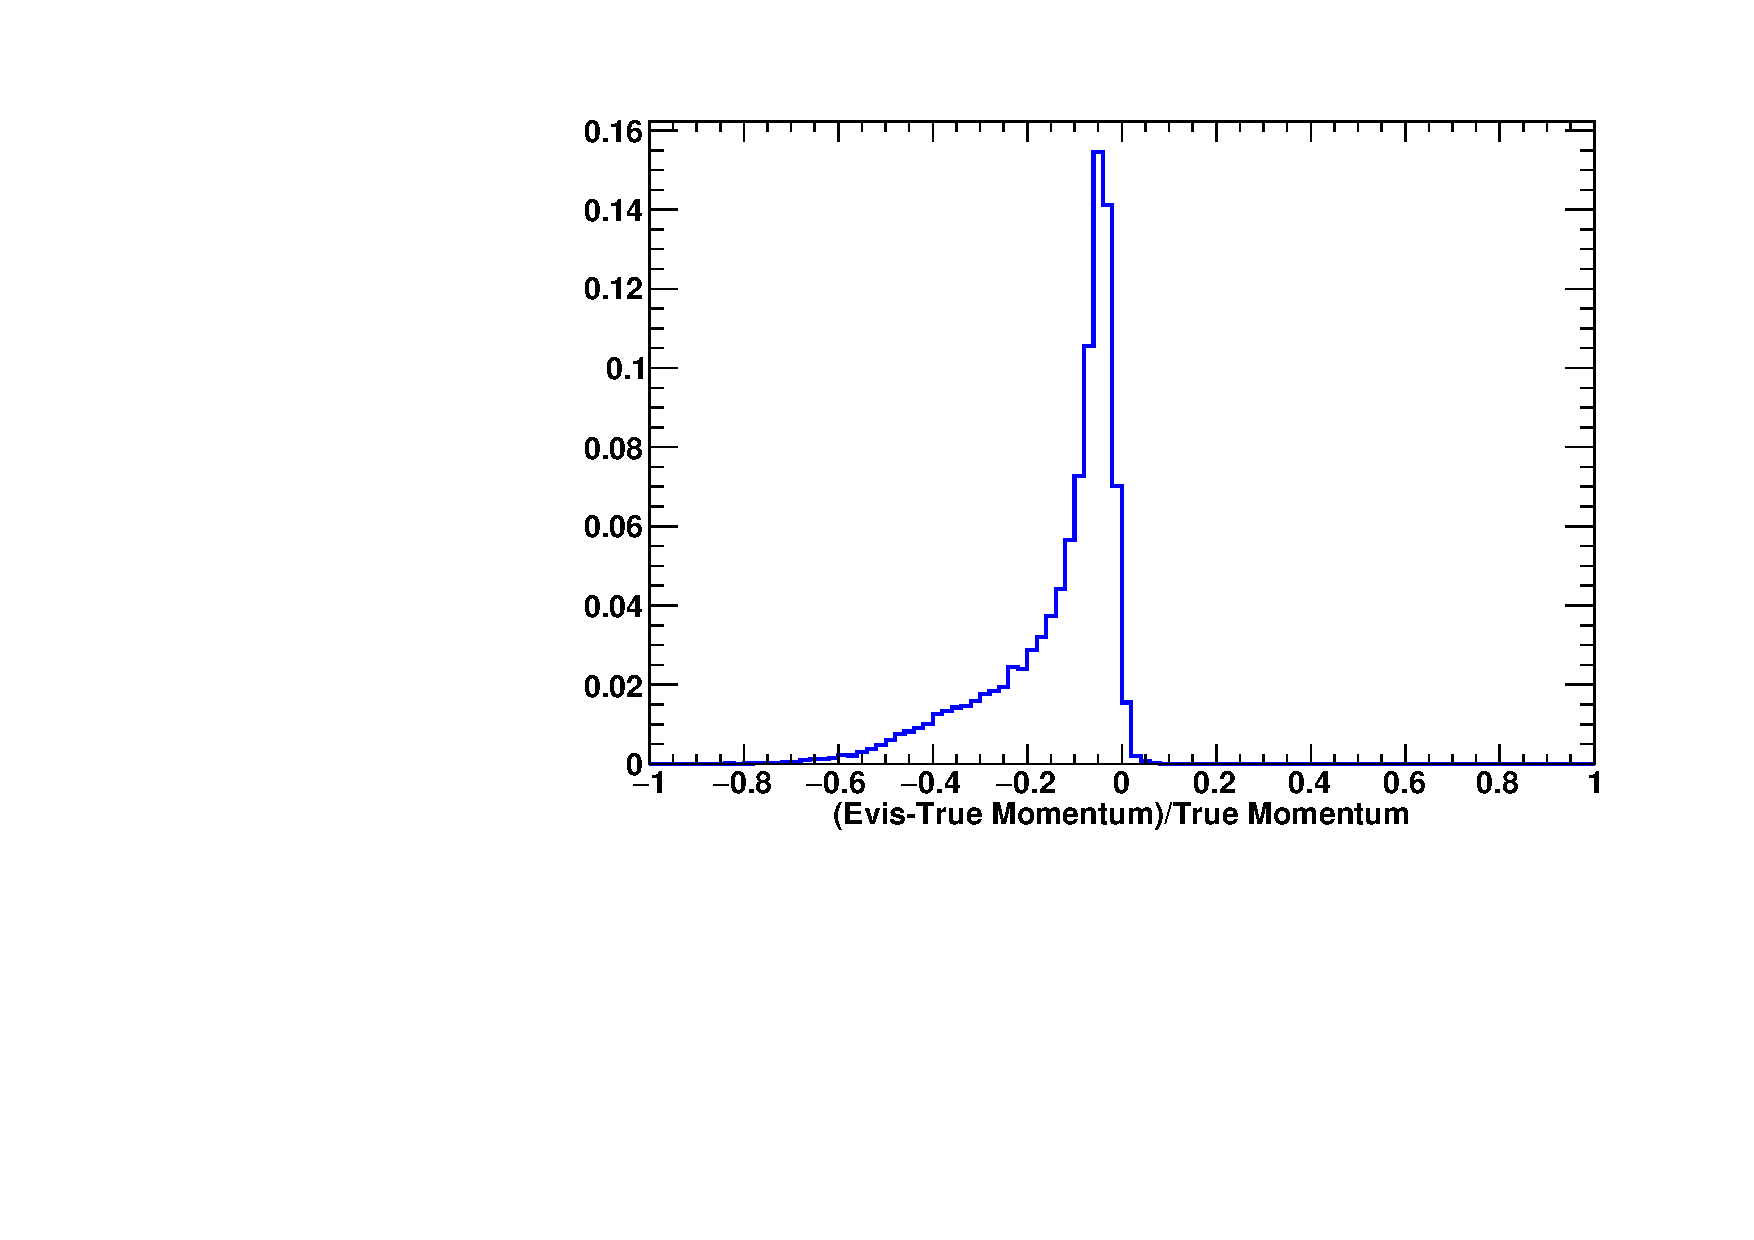
\includegraphics[width=0.3\textwidth]{figures/10GeV_100GeV_energy.pdf}
		\label{fig:energy_res_high}
	}
\caption{Energy resolution for events passing all selection and analysis cuts, from signal MC in 3 energy ranges.} 
\label{fig:energy_res}
\end{figure*}  

\begin{figure}
	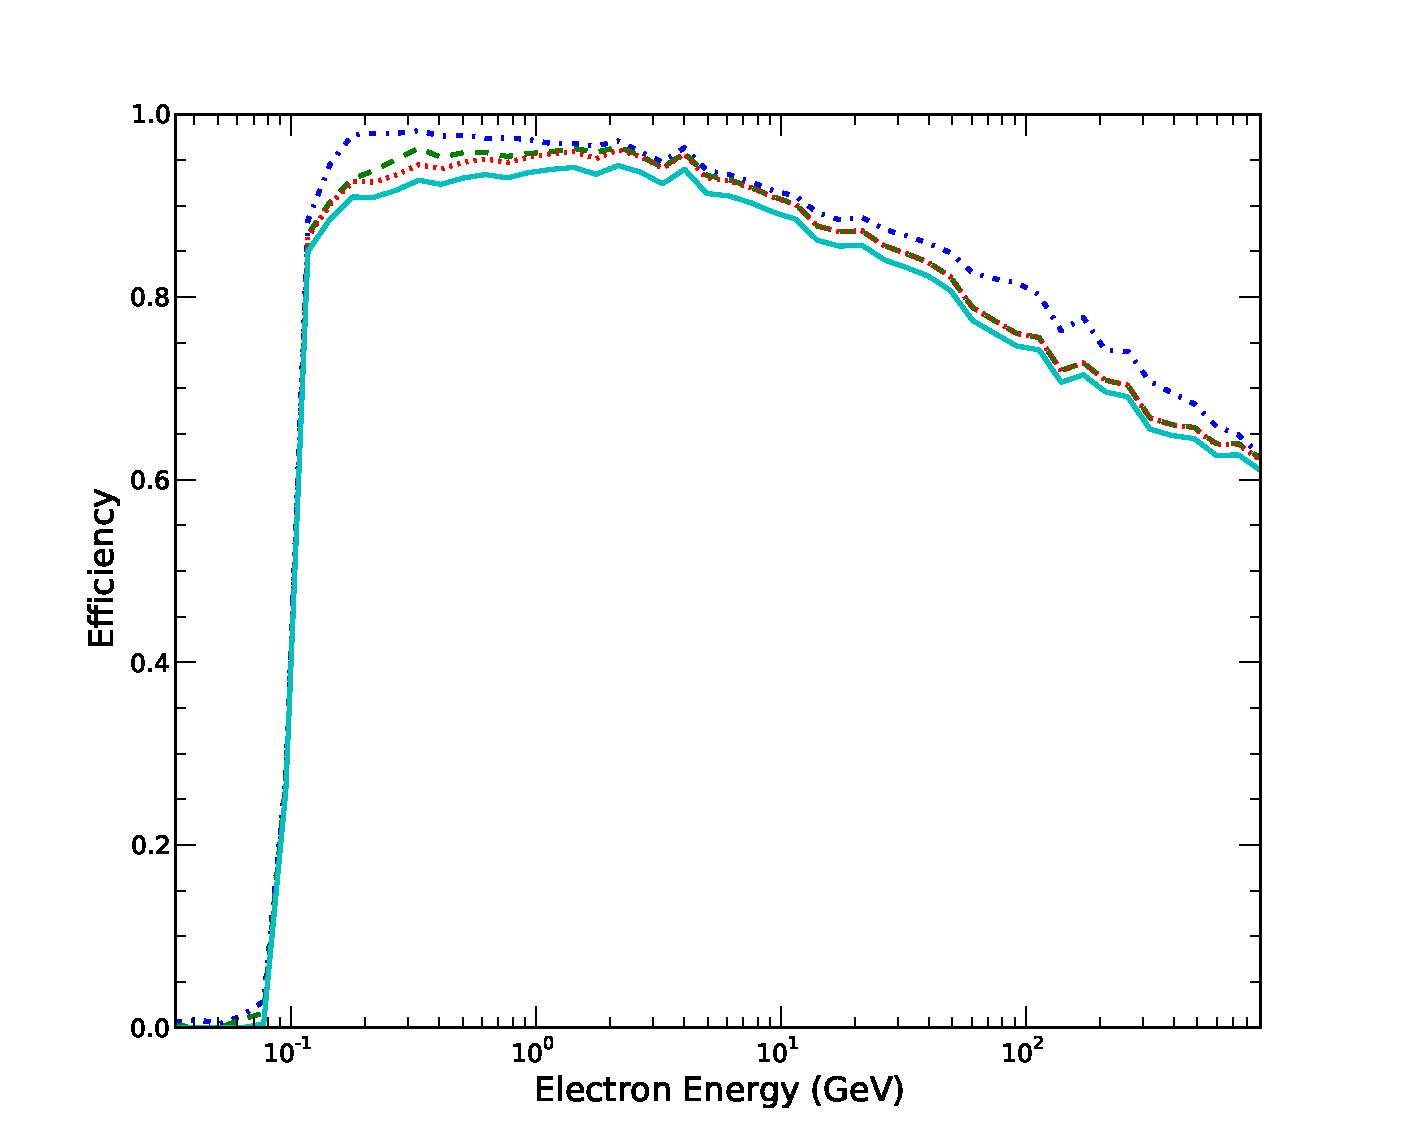
\includegraphics[width=0.6\textwidth]{figures/efficiency_30MeV_1TeV.pdf}
	\caption{Efficiency of the selection and analysis cuts as a function of energy.  Beginning with the FCFV reduction (dashed-dotted blue), the addition of the 1-ring (dashed green), e-like (dotted red) and finally 0 decay electrons and 0 tagged neutrons cuts to arrive at the final efficiency (solid cyan) are shown.  Note that the efficiency of the 0 decay electrons cut is $>99.99\%$, so that the drop from the dotted red line to solid cyan line is due solely to the background rate of the neutron tagging algorithm.}
	\label{fig:eff}
\end{figure}



 